\chapter{Introduction}
\label{chap:intro}

Methane is one of the most dominant greenhouse gasses (GHG) in the Atmosphere and behind CO$_2$, the second most important anthropogenic greenhouse gas. It has a Global Warming Potential Value (GWP) of 81 for a 20-year horizon \cite{Forster.2021}, making it 81 times more potent than CO$_2$ for that time interval \cite{T.Stocker.2013}.\\
Methane is released into the Atmosphere in large quantities. Estimations suggest 363 Mt annual emissions \cite{IEA.4262023}. Various sources produce methane and release it into the Atmosphere, ranging from natural to anthropogenic. Natural methane emitters are considered ones where humane influence is not directly involved, such as microbial decomposition of organic materials in wetlands, volcanic activities or bound methane releases in permafrost deposits due to temperature rise \cite{Fernandez.2022}.  Anthropogenic sources are usually connected to using, transporting and treating fossil fuels, such as natural gas or oil. Fugitive releases from gas pipelines contribute to methane emissions significantly \cite{Schwietzke.2014}, \cite{McKain.2015}, along with other chemical industries and human infrastructure. This includes wastewater treatment, landfills, agriculture, and livestock. The methane present in the Atmosphere is always a mixture of all the different emitter types, particularly in densely populated regions.\\
Identifying and quantifying these emitters is of utmost importance to understand and predict the mechanisms that govern climate change and subsequently be able to create informed legislation to rein in runaway emissions that can permanently harm the atmosphere's equilibrium. \\
Hamburg is the second-largest city in Germany, with a population of around 2.5 million. The city has various urban uses, including typical residential areas with high and low-density neighbourhoods and extensive industrial, commercial, and port spaces. These industrial areas also include oil and gas refineries. Additionally, the city also provides numerous natural environments like parks and gardens. The extensive network of rivers, channels, lakes, ports and wetlands is a unique feature for a city 70 km inland.  The most prominent water body is the river Elbe. The Elbe connects the city to the North Sea, providing Europe's third-largest port, the Hamburg port, with a year-round navigable offshore shipping route. It has a diverse system of methane emissions sources that contribute to the methane composition in the air.\\
It is known that the Elbe is a significant methane emitter \cite{Matousu.2019}. The methane concentration in its water and release of methane into the atmosphere varies for the entire river. Its uneven distribution originates from many factors that will be discussed in further detail.\\
The river originates in the "giant mountains" in the Czech Republic. The first section is a natural fast-flowing river experiencing no impact by human influences. The river has no significant methane emissions in this region as the natural methane oxidation mechanisms are balanced with its production and influx mechanisms. In the second section, the river is heavily industrially used in the Czech Republic. The river is severely impounded in this section. The water has a high methane concentration due to pollution and few natural regeneration areas that form the feeding ground for good microbial methane oxidation. \\
The Third section describes the Elbe as a lowland river flowing through Germany. Groynes only stabilize its banks, and the river is significantly naturalized with free-flowing characteristics. In this section, the microbial methane production is kept in check with its countering oxidation processes, resulting in a low methane concentration in the water and consequent low atmospheric diffusion rates.\\
Some heavily impounded human-made structures are present throughout the river, including harbours, locks, and weirs. These sections form methane hotspots, as methane production is rampant due to the disturbed flow of the river and heavy pollution. At the same time, the oxidating mechanisms are repressed. The reason for the inability of oxidation is not fully understood yet and is most likely a multifactorial cause \cite{Matousu.2019}, \cite{Bednarik.2019}.\\
The river Elbe estuary starting at the city of Hamburg, down to the North Sea into the Waddensea, experiences different environmental factors, and different mechanisms drive its methane production and reduction mechanism. The upper estuary, including Hamburg's port, is defined by the heavily impounded region around Hamburg and experiences significant variations in water level due to the Tide. While no significant methane transfer from the saltwater of the Waddensea to the very nutrient-rich freshwater occurs in the upper estuary due to insufficient mixing \cite{Matousu.2019}. The water in this region has a short turnover time, with a very high methane concentration, similar to other harbours and human-altered segments upstream. The water has high pollution and biomass concentration from industry, agriculture, and other human and natural influences upstream and in the region. This high concentration of pollutants and biomass significantly enhances the methane production mechanisms while hindering the Oxidation mechanisms. High heterotrophic activity is related to remineralization processes of high loads of labile organic matter, and it has been shown by \cite{Matousu.2019} that the methane concentration in the Upper estuary correlates with BOD-7 (a measure of bioavailability of degraded organic matter). \\
This is further amplified by its short turnover time, where the oxidation processes have little time to take effect and efficiently remove methane from the system.\\
The river is significantly widened in the lower estuary, with an extensive network of connected marshlands. The marshland has methanogenic bacteria that are well-adjusted to the colder climate of northern Germany. Those can be found in oxic as well as in anoxic soil layers. Resulting in a methane production peak at 10 °C and 20 °C. \cite{Wagner.1997} The low-temperature peak production occurs due to reduced methane oxidation at low temperatures. Marshlands systems usually peak in a 30 °C region in warmer climates. \\
The water turnover time is significantly longer, providing good conditions for methane oxidation and greater methane diffusion into the atmosphere, resulting in a ten times lower methane concentration than in the upper estuary \cite{Matousu.2019}. A significant amount of the methane in the lower estuary originates from the Waddensea, as the tides flush highly methane-enriched water into the estuary. The well-functioning oxidation processes in this region would otherwise dominate the methane balance.\\
Low water levels in the river and high temperatures enhance microbial activity and thus decrease oxygen levels in the water. This can, for example, be observed in the seasonal cycle. While no apparent relation to suspended particular matter can be seen, the sediment has a significant role in the methane cycle. For example, Methanotroph reduces CH$_4$ Emissions from the sediments.  As one can observe from tidal activities, resetting the sediments significantly increases methane production due to the reintroduction of biomass and ions to the sediments \cite{Bednarik.2019}. The types of methane-producing microbe can vary significantly due to the type of sediments and vary significantly throughout the river, allowing them to form hotspots.\\
The water level also contributes to the methane balance. Low water levels reduce the ability of the water to oxidize the methane due to its lower water column height over the sediments. In the Elbe estuary, the methane concentration in the water is correlated to falling water levels due to the Tide. It is reaching its peak at the lowest water level. \cite{Harrison.2017} have shown that the fast reduction of the water level increases the methane concentration and, consequently, its emission to the atmosphere. \\
A possible explanation is that the thick sediment layers can accumulate a large amount of methane. The drop in pressure due to the reduction in water column height causes the methane to form bubbles, which are released from the sediments and travel up to the surface and escape to the atmosphere. The reduced water column height can no longer oxidize most of this methane, consequently defusing the methane into the atmosphere. The exact condition required for such a surge in methane emission is not yet detailed. It is most likely a function of sediment characteristics, water depth, lowering rate, etc.\\
For the Elbe estuary, it is estimated that 5–41 \% of the total methane loss in the water is attributed to active methane oxidation. The remaining part is released into the atmosphere due to diffusion \cite{Matousu.2019}.\\
The United Nations environment programme (UNEP) measurement campaign aimed to quantify the emissions in the city region of Hamburg, Germany. While providing the opportunity to compare and validate different data acquisition approaches with the best bottom-up inventories currently available.\\
The campaign was conducted between 01.08.2021 and 1.04.2022, with some short 1-3 day maintenance breaks. High time-resolution mass spectrometer measurements were conducted during the campaign, focusing on Deuterium ($^2$H) and Carbon 13 ($^13$C) isotopes. The measurement was stationary on the roof of the Geomatikum building owned by Hamburg University near the city centre, with a measurement inlet height of 83 m \cref{TimelineNoPeaks}.
\begin{figure}[htbp]
 \centering
 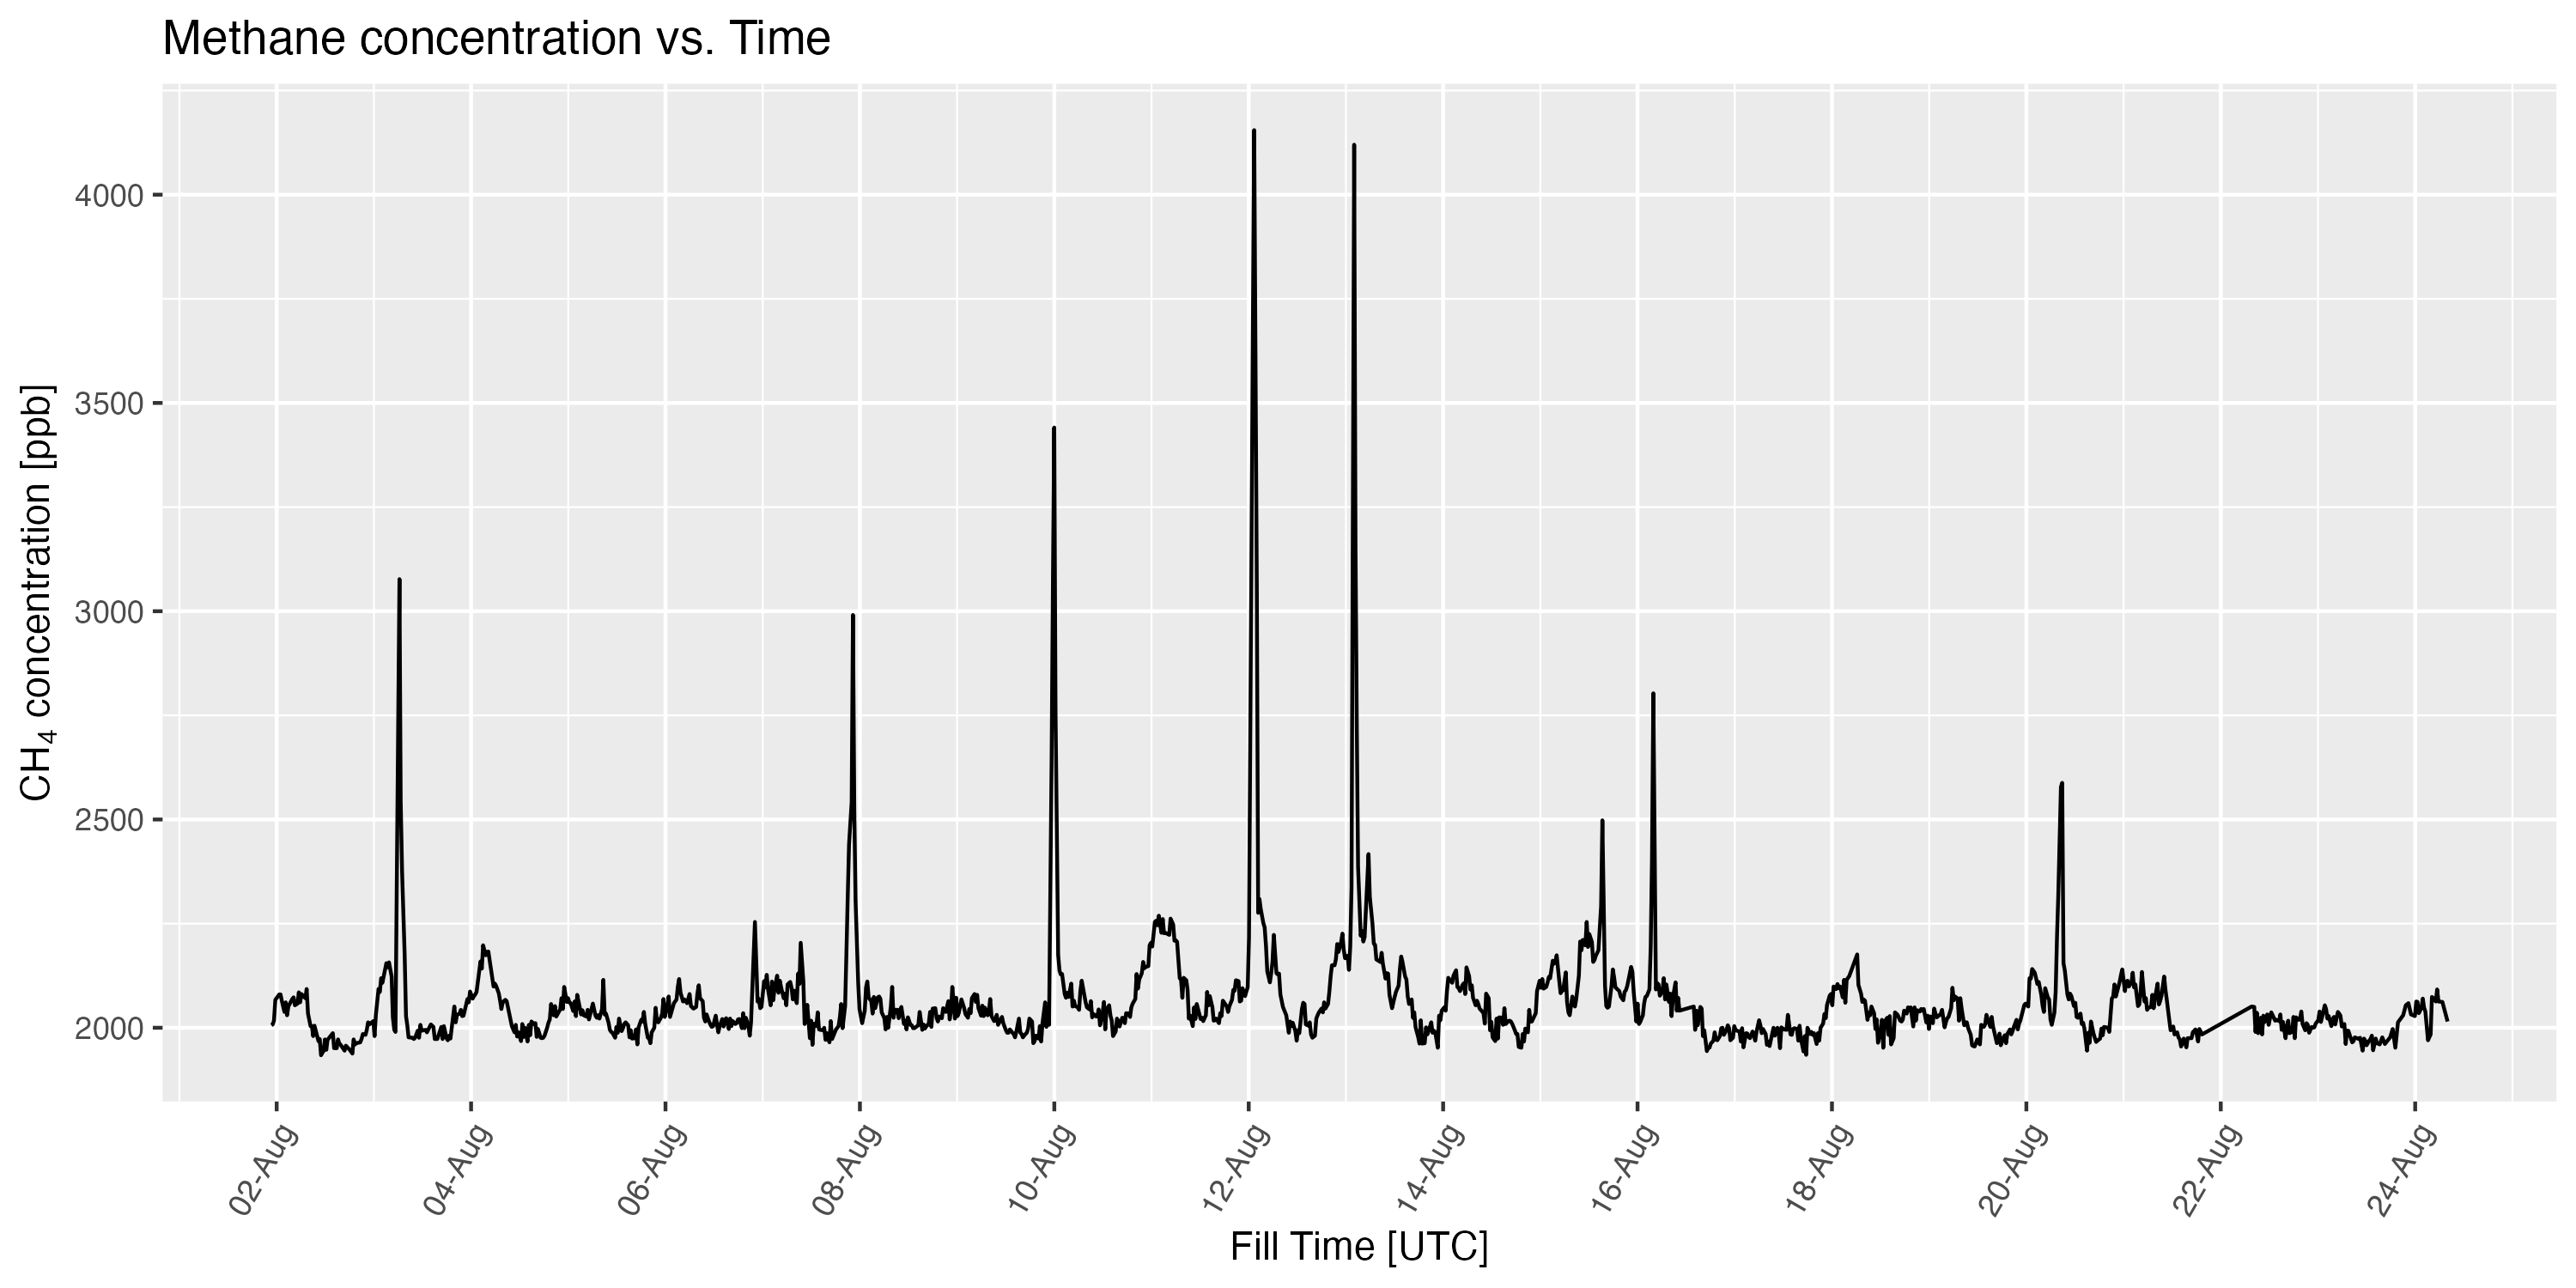
\includegraphics[width=1\textwidth]{figures/Appendix/CH4_Timelines/4_CH4_Timeline0_No_Peaks.png}
 \caption[CH$_4$ Timeline]{Section of CF-IRMS in situ measurement showing the timeline of methane concentrations measured in Hamburg Geomatikum (83m above ground) from 02.08.2021 to 24.08.2021.}
 \label{TimelineNoPeaks}
\end{figure}
A series of additional measurement approaches were conducted for the shorter period of 27.07.2021 to 9.09.2021. These include a solar-tracking Fourier Transform Infrared Spectrometer (FTIR) Network with four EM27/Sun spectrometers in and around Hamburg. This network enabled a differential total column measurement using the Bayesian inverse modelling approach. A Leosphere Windcube 200S Doppler wind LIDAR was also deployed to improve the transport modelling of the Bayesian inversion by correcting the atmosphere Boundary layer height and the wind direction of the wind model. \\
Mobile methane measurements by car and boat were also conducted to validate and improve the inventory for the uses as prior in the Bayesian inverse modelling.  A Picarro model G2301 measured mole fractions of CH$_4$, CO$_2$ and H$_2$ at a frequency of 0.3 Hz and a Picarro model G4302 measured mole fractions of C$_2$ H$_6$, H$_2$ O and CH$_4$ at frequencies of 1 Hz. The mobile measurements mainly focused on the industrial and port region in the south of Hamburg, filling the gaps left by a previous measurement campaign with the same approach, primarily focusing on the residential areas to the north.\\
The Isotope measurements and, to some extent, the FTIR measurement yielded some surprising results for their methane concentration that could initially not be explained. In particular, some seemingly randomly occurring high methane concentration peaks were observed. These peaks had a dry air mole fraction of up to 4500 ppb, while the average background was around 2000 ppb. The duration of the peaks was also concise, lasting for only around 0.5-3 h. The current global average mole fraction of methane is at 1921.74 ppb (January 2023) \cite{Lan.2022}.\\
By investigating the chemical composition of the methane by the Keeling method from Air sampled during the peaks, it was concluded that emission sources were due to natural microbial methane production mechanisms. Pointing towards wetlands and water bodies.\\
A purpose build particle transport model pointed towards emissions origination in the region of the city where the port, fleets, channels, and wetlands are located. \\
The occurrence of the peaks has been successfully correlated to the water level of the Elbe, as these regions experience strong water level fluctuations due to tidal effects. \cite{Harrison.2017} shows that a fast-dropping water level can trigger significant methane emissions into the atmosphere at freshwater reservoirs. Additionally, \cite{Matousu.2019} shows that the methane concentrations in the water of the river Elbe increase at dropping water levels.\\
Further correlations of meteorological and water quality data with the methane concentration in the Air provide an overall concrete conclusion of the origin of methane peaks. Linking it to the water bodies and wetlands in and around the city due to a complex interplay of man-made riverbank impoundments, pollution in the water, flow characteristics of the river sediment depositions and tidal influences.\\
The river Elbe is currently underrepresented in methane inventories. This is also suggested by \cite{Forstmaier.2023}, in which the methane modelling is significantly improved by including the river in the inventory. While the fluctuations of methane release by rivers and wetlands due to tidal effects are not well investigated and understood yet. This thesis shows their observable effects and the conclusion linking methane concentrations in the air to the river Elbe while providing ideas for further research.
